\documentclass{article}
\usepackage{multicol}
\usepackage{hyperref}
\usepackage{graphicx}
\usepackage[noend]{algpseudocode}
\graphicspath{ {./images/} }
\usepackage[utf8]{inputenc}
\usepackage{imakeidx}

\makeindex[columns=3, Index, intoc]

\usepackage{amsmath}
\numberwithin{equation}{section}
\renewcommand{\theequation}{Eq. \thesection.\arabic{equation}}


\title{\textbf{Progettazione e sviluppo di modulo raccolta dati e test suite automatica per intelligenze artificiali che si occupano di creare strategie di investimento}}
\author{Garion Musetta\\~\\garion.musetta@studenti.unimi.it}

\begin{document}
	\pagenumbering{arabic}
	\maketitle   
	\newpage
	\tableofcontents

	\newpage 
	 
	 
   	\section{Introduzione}
		Scopo di questo documento è affrontare il tema delle metodologie di test per intelligenze artificiali, descriverne alcune tecniche ed analizzare risultati ottenuti applicandole in uno specifico dominio.
		\\~\\
		Fra le diverse tipologie di intelligenze artificiali attualmente disponibili vengono considerate quelle di supporto alle decisioni, che si adattano particolarmente al problema e all'ambito in questione. Quando si sviluppa uno strumento di questo tipo è indispensabile porsi delle domande circa la qualità dei risultati prodotti dalla AI, confrontandoli con un modello ottimale di riferimento, che spesso non è disponibile oppure è molto difficile da produrre (in alcuni casi incalcolabile), e paragonandoli anche ad altre applicazioni già esistenti.


	\subsection{Descrizione dell'ambito di riferimento}
		Il dominio considerato è quello della finanza, in particolare lo sviluppo di strategie di investimento intelligenti.\\
		La AI in questione (\textbf{Sentyment}) è complessa e articolata, genera diverse strategie di investimento personalizzate per numerosi strumenti finanziari ed è anche in grado di piazzare direttamente ordini sul mercato, ovvero effettuare operazioni di acquisto e vendita. Il mercato in cui opera è quello delle criptovalute, in cui Bitcoin rappresenta in assoluto l'asset più famoso, ma è accompagnato da altre monete come Ethereum, Bitcoin Cash e Ripple, meno famose ma con le loro particolarità e altrettanto scambiate.\\
		L'obiettivo finale di Sentyment è produrre delle \textbf{strategie di investimento}: sono approcci di investimento personalizzati in funzione della propensione al rischio, degli obiettivi e degli interessi specifici del singolo investitore. Seguendo tale strategia, l’investitore può decidere sui diversi tipi di attività da includere nel proprio portafoglio di investimento. Una specifica strategia di investimento può essere determinata da una serie di fattori, come la propensione al rischio e i rendimenti che si vogliono perseguire sugli investimenti, nonché le attività, le regioni e i settori a cui si è interessati. Anche il periodo per il quale si intende investire contribuisce a configurare la strategia.\\
		Definita una certa strategia, Sentyment la persegue decidendo quindi, in ogni "istante di tempo" quale delle 3 possibili operazioni effettuare: \textbf{buy} (comprare il titolo azionario), \textbf{sell} (vendere) o \textbf{hold} (mantenere il portafoglio). Lo scopo a lungo termine della strategia è massimizzare il guadagno rispetto a quanto investito, oltre a rispettare i vincoli di rischio e interessi specifici dell'investitore. La AI è in grado di decidere quali fra queste operazioni effettuare al fine di massimizzare gli obiettivi.\\
		Le decisioni non sono prese esattamente "istante per istante": il periodo di tempo considerato è l'ora. Ogni ora la piattaforma di trading di riferimento produce nuovi dati e questi sono disponibili per essere scaricati dai trader, che possono quindi compiere le azioni sopra descritte. Oltre alla cadenza oraria è anche possibile scegliere i minuti: 1, 5, 15, 30, 60, 240, 1440, 10080, 21600 (dipende dalla piattaforma di trading).\\
		

	\subsection{Modello dei dati}
		Tutti i dati usati dalla AI sono scaricati da una piattaforma di trading, \textbf{Kraken}, un sito per lo scambio di criptovalute. Ogni secondo, trader da tutto il mondo effettuano azioni di compravendita di titoli, esattamente nel modo in cui opera anche Sentyment, facendo crescere o diminuire il valore azionario di ogni asset. Kraken rende disponibile, attraverso delle API, lo storico degli scambi effettuati per ognuno degli asset che espone (110 coppie di valute che rappresentano i valori di scambio fra criptovalute e USD / EUR ): si fa distinzione fra dati "RAW", ovvero un semplice elenco di prezzi variabili nel tempo, e le \textbf{candele OHLCV}. Le candele sono uno degli strumenti grafici più popolari in quanto offrono un eccellente riferimento virtuale dei movimenti dei prezzi in un intervallo di tempo ad un minuto, orario, giornaliero, mensile ed altro.
		\\~\\		
		Le candele ohlcv sono quindi la rappresentazione di un dato aggregato ora per ora (o secondo altre unità di tempo come minuto o giorno). Le informazioni che racchiudono sono indicate dal loro nome: open, high, low, close, volume. Prendendo come esempio le candele orarie: la creazione di ognuna di esse parte allo scoccare dell'ora e fissa un prezzo di apertura (open: il prezzo di vendita dell'asset in quel momento), per terminare dopo un'ora con un prezzo di chiusura (close: lo stesso prezzo di vendita dell'asset al momento di chiusura, che sarà ora cambiato rispetto a open); si calcola quali sono stati i picchi massimi e minimi di prezzo durante l'ora (high, low) e infine il volume, che rappresenta l'ammontare totale scambiato nell'ora.\\ Le candele OHLCV rappresentano quindi la 'storia' dell'andamento dei prezzi di un certo asset durante il periodo di tempo fissato: iniziano con un certo prezzo, che evolve toccando un minimo e un massimo, e termina con un certo prezzo di chiusura; i prezzi minimo e massimo possono superare anche di molto quelli di apertura e chiusura. E' anche possibile il caso in cui il prezzo non evolve e open, high, low e close coincidono.\\ Volume, invece, rappresenta la somma totale della quantità di titoli mossi durante l'unità di tempo.
		\\~\\
		
		
		\textbf{ESEMPIO NUMERICO CREAZIONE CANDELE???}
		(es, elenco prezzi in un'ora - > risultato candela valori ohlcv)
		\\~\\
		
		La AI lavora quasi esclusivamente sulle candele e, anche se le API di kraken permettono di scaricare dati già aggregati, Sentyment scarica soltanto dati di trading raw e poi crea autonomamente le sue candele attraverso un modulo dati dedicato.
		\\~\\
		

		\begin{figure}
		\begin{center}
		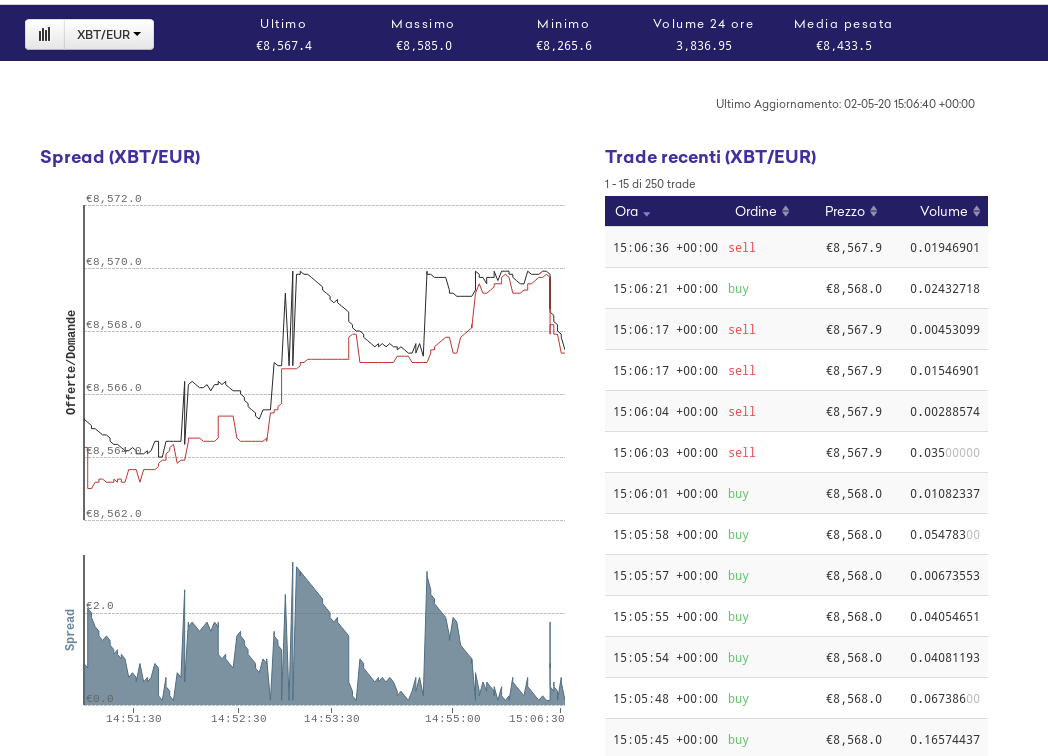
\includegraphics[width=10cm]{kraken_raw}
		\caption{\\~\\Elenco transazioni Bitcoin/Euro relative ad una finestra di minuti. I record mostrano l'ora in cui è avvenuto il trade, il tipo di operazione (buy / sell), il prezzo di scambio del titolo e la quantità di titoli scambiati. L'elenco dei dati 'raw' di trade è disponibile tramite le API kraken ed è la fonte grezza di dati finanziari utilizzati per calcolare i grafici OHLCV, fondamentali per l'analisi dei mercati. (fonte: https://www.kraken.com/)}
		\end{center}
		\end{figure}
		\begin{figure}
		\begin{center}
		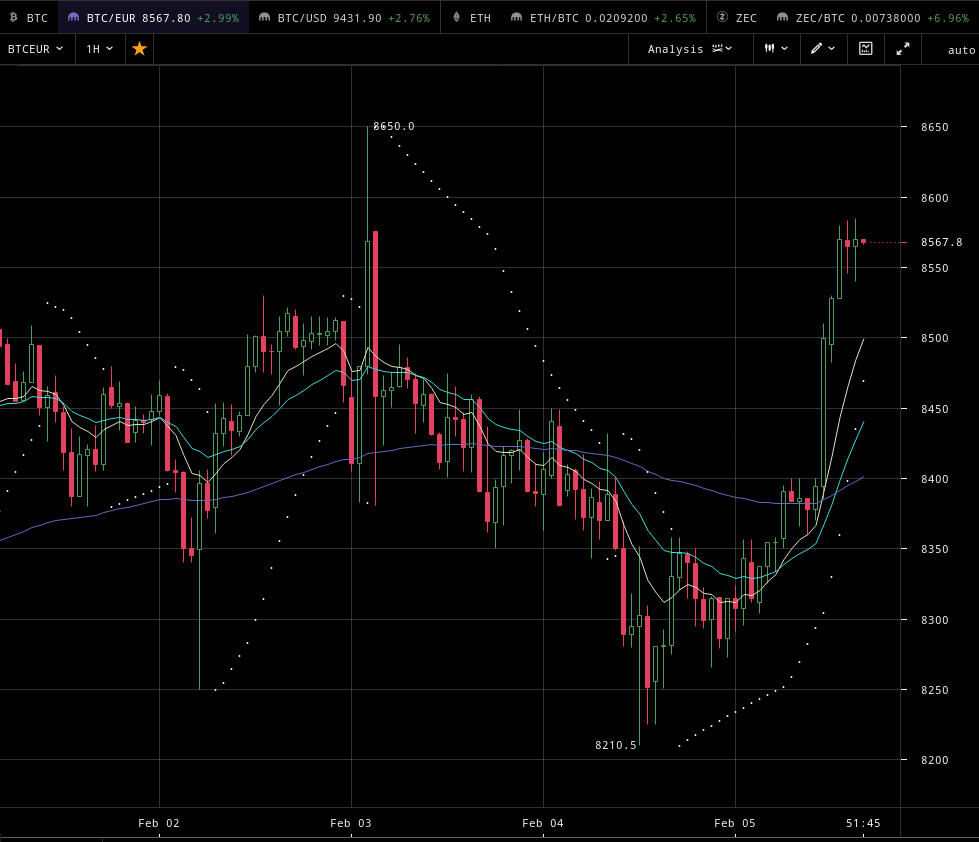
\includegraphics[width=\linewidth]{kraken_ohlcv}
		\caption{\\~\\Grafico OHLCV ricavato dai prezzi in Figura 1. Le candele sono di durata 1 ora e quindi i prezzi elencati sopra rientrano soltanto in parte nell'ultima candela (rossa) delle 15:00 - 16:00, ancora aperta e quindi in creazione. La candela è rossa perchè, come si nota dai prezzi, il valore del titolo  è in discesa: partendo da circa 8.568 (probabilmente più alto nei record precedenti) si scende verso 8.567.\\~\\Le linee colorate rappresentano le medie mobili dei prezzi di chiusura; usate per analisi tecnica, sono rispettivamente le medie a 10 (verde), 21 (azzurro= )e 100 (blu) candele. Più candele sono considerate nella media e meno questa cambierà bruscamente, avendo quindi la media a 100 candele (cioè 100 ore) molto più lenta delle altre. (fonte: https://www.kraken.com/)}
		\end{center}
		\end{figure}

		
		
		Le immagini descrivono l'andamento dei prezzi, scambio per scambio, e le corrispondenti candele ohlcv come esposte dalla piattaforma di trading. I bordi orizzontali che compongono i lati superiore e inferiore della candela sono il prezzo di apertura e quello di chiusura: se la candela è rossa il prezzo di chiusura è minore di quello di apertura (significa che il prezzo dell'asset è sceso durante l'unità di tempo), e quindi il bordo superiore sarà 'open' e quello inferiore 'close', mentre una candela verde indica una crescita del prezzo ('open è il lato inferiore mentre 'close' quello superiore). Le linee verticali della candela si estendono invece verso il prezzo minimo e massimo che l'asset ha toccato nel periodo di tempo fra apertura e chiusura della candela.
		\\~\\
		Le API di Kraken permettono di effettuare diversi tipi di operazioni, come scaricare lo storico dei prezzi di tutte le coppie valuta-criptovaluta disponibili, così come ricevere in tempo reale i nuovi dati sugli scambi di titoli. Inoltre è anche possibile, sempre tramite API, creare il proprio portafogli sulla piattaforma e piazzare ordini di acquisto e vendita; tutte funzionalità ben sfruttate da Sentyment, che opera sul mercato in autonomia.
		
		
		
	\subsection{Gudagnare con trading}
		E' importante notare innanzitutto che la ricchezza in possesso, calcolata in ogni istante, è data non soltanto dalla quantità di budget, ma anche dalla quantità di titoli posseduti. Gli asset finanziari hanno un valore monetario indicato dal loro prezzo e quindi il possesso di alcuni di questi, anche se il budget da investire è azzerato, comporta comunque una ricchezza investita che si può recuperare vendendo il titolo.\\
		Esempio asset XBT/EUR, valuta di scambio fra Bitcoin e Euro. Partendo da un certo budget iniziale in Euro, si decide quando comprare titoli di Bitcoin e quando rivenderli per avere di nuovo Euro. Lo scopo quindi è non soltanto massimizzare gli Euro in possesso, con l'avanzare del tempo, ma anche i Bitcoin e / o una combinazione dei due titoli che porti comunque ad un aumento del valore dei due.\\
		A seconda dell'aspettativa di rialzo o ribasso del titolo: andare \textbf{long} su XBT/EUR vuol dire acquistare Bitcoin vendendo Euro, puntando ad un apprezzamento (aumento di valore) della criptovaluta; in questo caso l’aspettativa è di un aumento del valore del cambio e si avrà quindi una visione rialzista del mercato. Andare \textbf{short} su XBT/EUR vuol dire vendere Bitcoin acquistando Euro, puntando quindi un apprezzamento dell'Euro nei confronti della criptomoneta. In questo caso l’aspettativa è di una diminuzione di valore del cambio. Si aprirà quindi una posizione che mira a una flessione del prezzo. La visione che il trader avrà del mercato sarà ribassista.\\~\\
		Il punto centrale su cui si basano le strategie di investimento è cercare di indovinare se la valuta aumenterà o diminuirà di prezzo, per poi andare long o short a seconda della previsione. l'\textbf{analisi tecnica} è un metodo riconosciuto e largamente utilizzato per anticipare o prevedere l'andamento dei prezzi e si basa sull'aspetto tecnico del mercato, utilizzando grafici e dati storici. In particolare vengono analizzati prezzi, volumi scambiati e fasce temporali. Si utilizzano indicatori matematici, statistici e grafici e i segnali e i suggerimenti ricavati da questi strumenti accompagnano i trader nelle loro decisioni in merito all'apertura e chiusura di posizioni di trading. L'analisi tecnica è un metodo di previsione dei prezzi basato sui dati storici.
		\\~\\
		\textbf{Altro su analisi tecnica? https://www.xtb.com/it/scuola-di-trading/che-cosa-e-lanalisi-tecnica}
		\\~\\
		Supponendo che il mercato ad un certo punto cresca e si abbia "indovinato" un buon numero di previsioni, ci si ritroverà a possedere dei titoli che ora valgono un prezzo superiore rispetto al loro valore iniziale. Se i titoli crescono di valore, è bene quindi acquistarne finchè salgono, in questo modo si possiede un maggior numero di asset che andranno a valere sempre di più; in caso di perdita di valore del titolo, invece, generalmente si dovrebbe vendere i titoli, per riacquistare del budget investito che ora stava perdendo valore e poterlo investire in altri titoli che crescono.\\
		Quando si decide di acquistare si sta effettuando la seguente operazione: dato un certo budget iniziale \textit{budget}, il valore del titolo \textit{price} e la quantità di titolo acquistato \textit{equity} e supponendo di spendere sempre tutto il budget per acquistare il titolo
		\\
		
		\begin{equation}
			equity=budget/price
		\end{equation}
		\\~\\
		Mentre, all'occorrenza di un'operazione di vendita, utilizzando equity appena acquistata:\\

		\begin{equation}
			budget=equity*price
		\end{equation}

		\\~\\
		È possibile in ogni momento calcolare il ricavo o quantità di beni in possesso combinando il budget con equity, tenendo presente che dopo un acquisto il budget scende a zero e equity assume il valore indicato, mentre dopo una vendita è equity a scendere a zero e si ritorna in possesso di budget. Lo stesso budget riacquistato verrà usato nuovamente per comprare dei titoli facendo così crescere di nuovo equity, e così via. Un vincolo è quello di non poter effettuare due medesime operazioni di fila: 
		\\~\\
		Se si considera un certo budget iniziale \textit{initial\_budget}, il \textbf{guadagno} (\textit{gain}) in ogni istante è dato da:
		\\
		\begin{equation}
			gain=(budget+equity*price)-initial\_budget
		\end{equation}

		\\~\\
		Questa è la formula del guadagno che verrà usata da qui in avanti.		
		\\~\\\\~\\
		A questo punto è necessario introdurre il concetto di \textbf{fee}.\\
		Le varie piattaforme di trading addebitano un costo per ogni singola operazione, sia di acquisto che di vendita, intestandosi una percentuale di budget speso dai trader come tassa per mantenere la piattaforma stessa. Nel caso di operazioni di acquisto, la tassa è calcolata come percentuale del budget speso per comprare il titolo, quindi viene scalata subito e il risultato è l'acquisto di una quantità leggermente minore di titoli (la restante dei quali viene pagata alla piattaforma); per le vendite invece la fee è tolta dal budget una volta che questo è ricalcolato vendendo equity, risultando in un ricavo leggermente minore di quello che si sarebbe ottenuto vendendo realmente l'intera quantità di titoli.\\
		Nel caso di Kraken, la piattaforma di trading di riferimento su cui opera Sentyment, le fee sono del 0.26\%: significa che viene sottratto il 0.26\% di budget che si intende investire, per ogni operazione. Per altri mercati, valute o piattaforme di trading le fee possono variare e potrebbero non essere basaste su una percentuale di acquisto ma fisse (flat fee vs per share fee).
		\\~\\
		La presenza delle fee modifica abbastanza drasticamente il funzionamento del mercato e l'efficacia delle strategie di investimento, che devono essere adattate ad un mercato con fee; è necessario quindi riscrivere le formule per il guadagno e per le operazioni di acquisto e vendita titoli, che ora comprendono la percentuale di fee.\\
		Per gli acquisti, considerando un certo budget iniziale \textit{budget} (o il budget risultato di una precedente vendita), il valore del titolo \textit{price}, la quantità di titolo acquistato \textit{equity} e una tassa \textit{fee}:\\
		\begin{equation}
			equity=(budget*(1-fee))/price
		\end{equation}
		\\~\\
		Per le vendite:\\
		\begin{equation}
			budget=(equity*price)*(1-fee)
		\end{equation}
		\\~\\
		Dal momento che le budget e equity sono già calcolati togliendo le fee per ogni operazione di acquisto e vendita, la formula del guadagno rimane la stessa.\\~\\
		
		
		
		
		
		
		
		
		\textbf{ESEMPIO DI COME CAMBIEREBBE RISULTATO CON E SENZA FEE CON POCHI DATI DI ESEMPIO?}
		\\~\\
		
		
		
		
		
		
		
		
		
		
		Senza addentrarsi nelle diversità dei titoli e dei mercati, si può affermare che una strategia generale e semplificata per guadagnare facendo trading è dunque "compra basso, vendi alto"; nella realtà i segnali di acquisto possono essere dati da altri indicatori più complessi e non sempre è possibile capire quando un titolo sta toccando un prezzo particolarmente alto o basso: è facile analizzare i grafici "a posteriori", ma non altrettanto semplice prevedere massimi e minimi locali online. Per questo si utilizzano delle semplici strategie fondamentali che aiutano a capire l'andamento dei prezzi.
		
		
	\subsection{Esempi di strategie}
		Come già accennato, l'\textbf{analisi tecnica} è lo studio dell'andamento dei prezzi dei mercati finanziari nel tempo, allo scopo di prevederne le tendenze future, mediante principalmente metodi grafici e statistici. In senso lato è quella teoria di analisi secondo cui è possibile prevedere l'andamento futuro del prezzo di un bene quotato, studiando la sua storia passata. Viene utilizzata, assieme all'analisi fondamentale, per la definizione delle decisioni di operatività finanziaria.\\
		L'analisi tecnica si prefigge di analizzare e comprendere, attraverso l'analisi del grafico, l'andamento dei prezzi, il quale a sua volta rispecchia le decisioni degli investitori; inoltre si basa sull'assunto fondamentale che, poiché il comportamento degli investitori si ripete nel tempo, al verificarsi di certe condizioni grafiche, anche i prezzi si muoveranno di conseguenza. Il compito principale dell'analisi tecnica è quindi quello dell'identificare un cambiamento di tendenza rispetto ad uno stadio iniziale, mantenendo una posizione di investimento fino a quando non vi sia prova che la tendenza stessa si sia di nuovo invertita.\\
		Per individuare un trend si fa uso di indicatori tecnici, basati su prezzo e volume, calcolati a partire dai grafici: questi analizzano i movimenti di prezzo a breve termine e alcuni dei più noti e usati sono Moving Average Crossover, MACD (moving average convergence / divergence), RSI (relative strength index) e Bollinger Bands.\\
		Analizzando i grafici passati mediante queste strategie è possibile ricavare i parametri per gli indicatori che meglio si adattano al mercato in analisi e riutilizzare l'indicatore, applicandolo ai dati futuri, per identificare i trend.\\~\\
		
		\subsubsection{Moving Average Crossover}
		Questa strategia prevede il calcolo di una o più medie mobili a diverso periodo, le cui intersezioni nel grafico definiscono un segnale di buy o sell.\\
		Il moving average crossover si verifica quando, nel grafico di due medie mobili ciascuna basata su diversi periodi, le linee di queste medie mobili si incrociano. Non prevede la direzione futura ma mostra le tendenze. Questo indicatore utilizza due (o più) medie mobili, una più lenta e una più veloce. La più veloce è una media mobile a breve termine. Per i mercati azionari di fine giornata, ad esempio, può essere un periodo di 5, 10 o 25 giorni mentre la più lenta è la media mobile di medio o lungo termine (ad esempio periodo di 50, 100 o 200 giorni). Una media a breve termine è più veloce perché considera i prezzi solo per un breve periodo di tempo ed è quindi più reattiva alle variazioni giornaliere dei prezzi. D'altra parte, una media mobile a lungo termine è considerata più lenta in quanto incapsula i prezzi per un periodo più lungo, tuttavia tende ad attenuare i disturbi che si riflettono spesso nelle medie mobili a breve termine.
		\\
		Una moving average, come una linea a sé stante, viene spesso sovrapposta nei grafici per indicare l'andamento dei prezzi. Un crossover si verifica quando una media mobile più veloce (cioè una media mobile di periodo più breve) attraversa una media mobile più lenta (cioè una media mobile di periodo più lungo). In altre parole, accade quando la linea della media mobile del periodo più breve attraversa una linea della media mobile del periodo più lungo: questo punto di incontro viene utilizzato per comprare o vendere titoli (quando la media veloce supera quella lenta, si ha un segnale di \textit{buy}, mentre \textit{sell} se viceversa)
		\\~\\
		\begin{figure}
		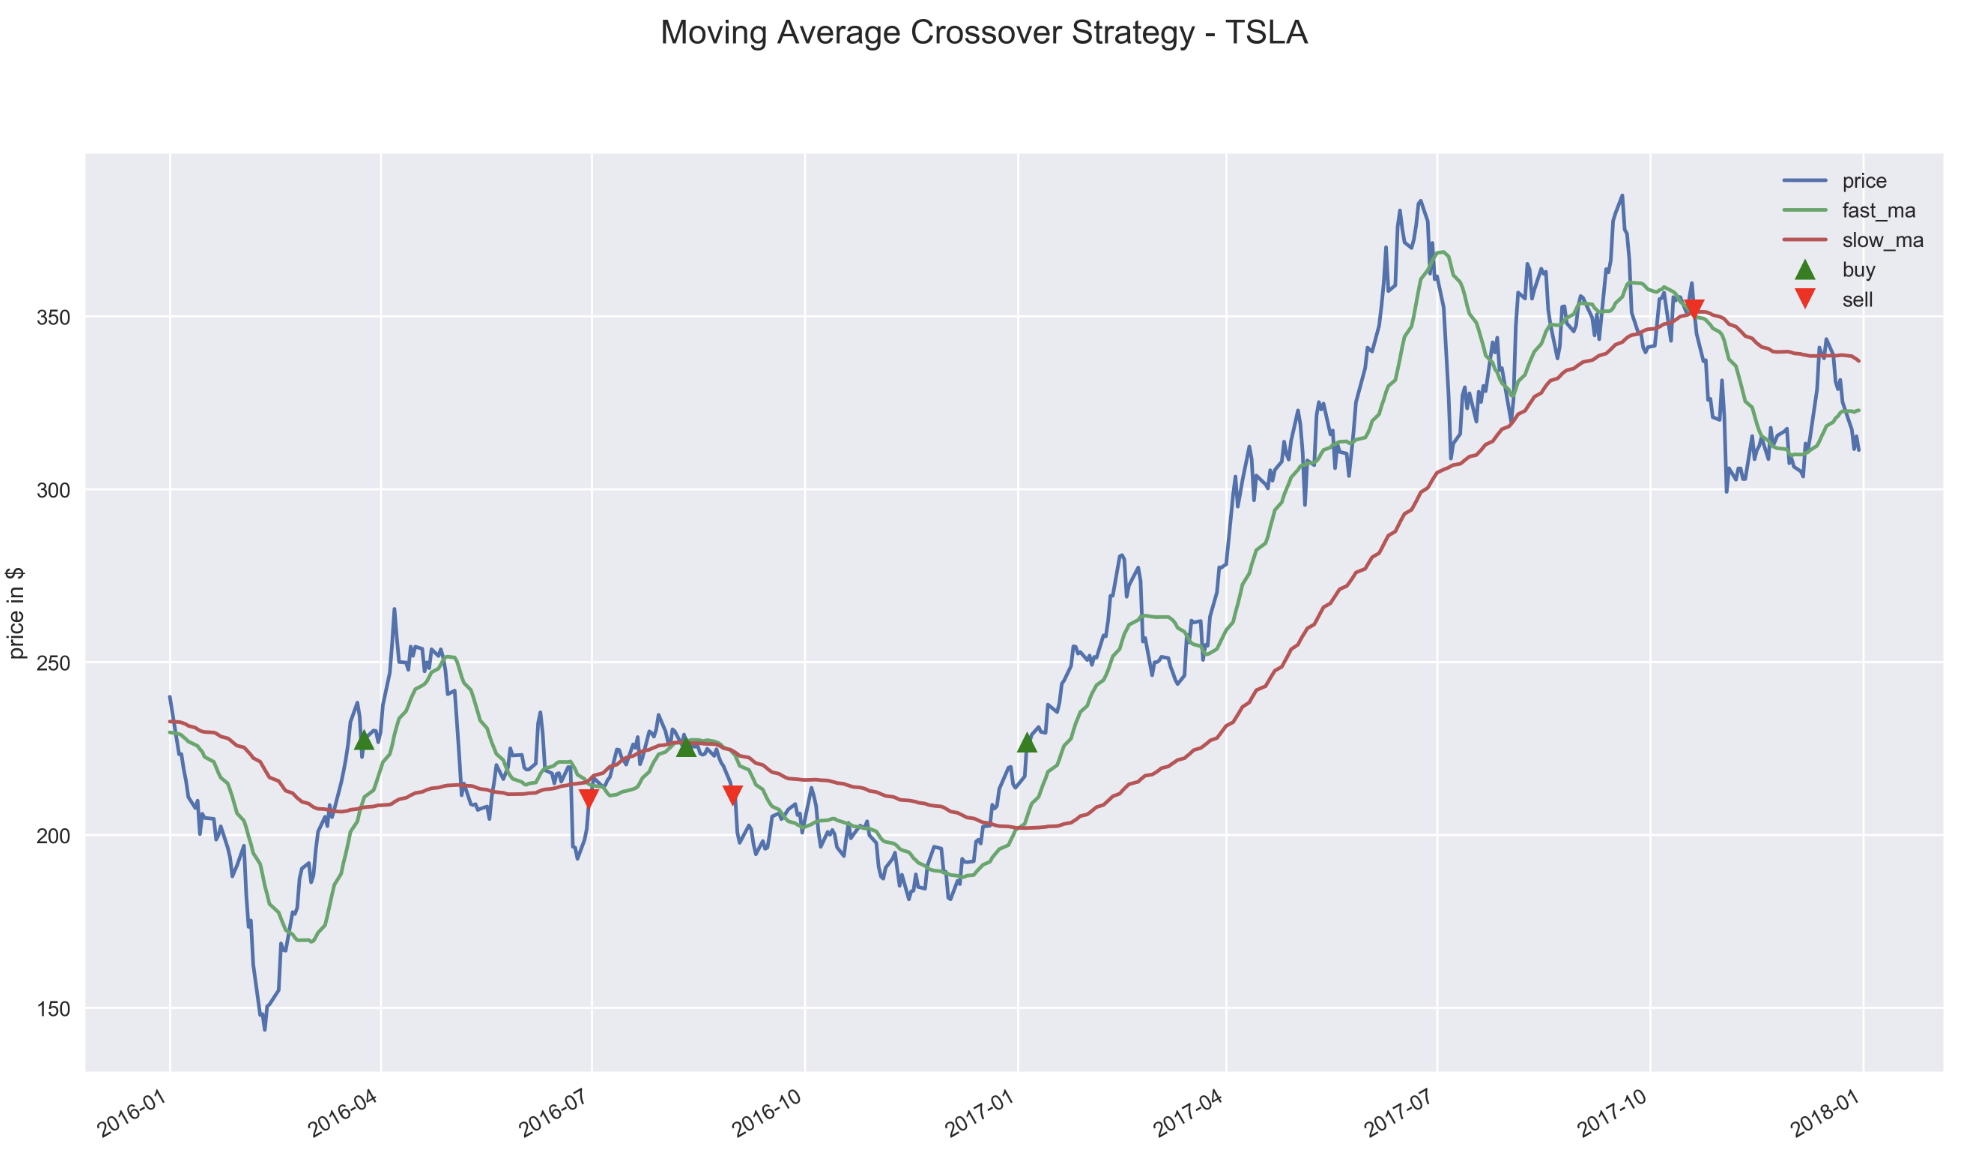
\includegraphics[width=\linewidth]{moving_avg}
		\caption{Andamento dei prezzi per il titolo TESLA/DOLLARO, accompagnato da due medie mobili a diverso periodo: fast\_ma a 20 giorni mentre slow\_ma a 100 giorni. Le frecce verdi e rosse indicano i segnali di buy e sell ricavati dalle intersezioni fra le medie}
		\end{figure}
		\\~\\
		Ci sono diverse declinazioni della strategia a medie mobili, come ad esempio SMA (simple moving average), che utilizza come segnale di buy / sell il crossover fra i prezzi di chiusura e la media mobile semplice; EMA usa una media esponenziale; MACD (moving average convergence / divergence) usa come prima statistica la differenza fra la media veloce e quella lenta e, come seconda statistica, la media di queste differenze.
		\\\textbf{PARLARE DI TUTTE LE STRATEGIE? MACD, RSI, BOLLINGER?}
		\\~\\
		Calcolati gli indicatori statistici più adatti alla situazione e scelti i parametri migliori (come i periodi delle medie da usare), si è costruito un modello di trend del titolo e si è in grado di prevedere quando il trend si ripropone. Prendendo l'esempio di una moving average crossover con una media veloce e una lenta, analizzato che per la maggior parte dei casi si riscontra un guadagno vendendo quando la media lenta supera quella veloce e comprando quando accade l'opposto, allora si può affermare che sarà molto probabile guadagnare ancora, in futuro, ripetendo le medesime operazioni.
		
		
	\subsection{Ruolo delle intelligenze artificiali e scopo della tesi}		
	L'apprendimento automatico e diverse tecniche hanno creato nuovi sistemi per individuare pattern, cosa che il cervello umano non è in grado di fare. Dal momento che la finanza è quantitativa, la AI nel trading azionario sta guadagnando terreno. Le società finanziarie hanno investito molto nell'intelligenza artificiale in passato e studiano e implementano le applicazioni finanziarie di machine learning e del deep learning nelle loro operazioni.\\
	L'analisi tecnica è dunque implementata in sistemi automatici, che sono molto più efficienti di un trader umano e offrono diversi vantaggi. Le AI separano le informazioni prevedibili da qualsiasi "rumore casuale", gli algoritmi apprendono dall'accuratezza delle previsioni precedenti e si adeguano continuamente, abbastanza veloci da prevedere il mutamento della situazione del mercato anche in un orizzonte di pochi giorni. Possono imparare dai successi e fallimenti e riconfigurare ogni giorno le approssimazioni del funzionamento interno del mercato, poiché viene alimentato con nuovi dati.\\
	Oltre agli indiscutibili vantaggi computazionali di una macchina rispetto al cervello, ci sono altri aspetti da considerare che hanno portato alla crescita delle AI nel settore. Si può infondere la conoscenza degli esperti dell'ambito in un software che si auto adatta e migliora, senza avere gli svantaggi dell'errore umano; si può estendere per permettergli di gestire diversi ambiti, dal recupero della materia prima (i dati di trading) fino alla vendita del prodotto finito (vendita di strategie di investimento). È possibile costruire sistemi complessi che modellano intere realtà umane.\\~\\
	Sentyment è uno di questi software descritti. Si occupa di raccogliere dati, elaborarli e, attraverso una AI li analizza per produrre strategie di investimento. Il modulo di intelligenza artificiale è molto ampio: esistono molte AI che operano producendo costantemente nuovi segnali di buy / sell per le strategie e sono monitorate da una ulteriore, singola AI. Questo supervisore decide quale fra le molte AI sta avendo più successo e la promuove come attiva da utilizzare.\\
	Lo scopo della tesi è sviluppare il supervisore e inserirlo all'interno del complesso sistema di Sentyment, impiegando tecniche di test per intelligenze artificiali che permettano di scegliere un rappresentante migliore fra una serie di agenti che operano indipendentemente.
	
	
	\newpage
	\section{Sentyment}
		Sentyment è un organismo ampio, formato da numerosi componenti interconnessi come, per esempio:
		\begin{itemize}
			\item Modulo raccolta dati
			\item Test suite
			\item Modulo di trading
		\end{itemize}
	
	
		Sviluppo modulo dati da me.
		
		Sentyment è composta da tante AI e vengono scambiate spesso; obiettivo finale della tesi è saper dire quando scambiare una con l'altra. (grazie ai test)
	    
	\newpage
	\section{Metodologie di test per intelligenze artificiali}	
	\subsection{Stato dell'arte dei test}
	\subsection{Analisi offline: maximum profit e genetic AI}
	\subsection{Analisi online: reinforcement learning}
	
	\newpage
	\section{Risultati}
		
	\newpage
	\cite{es}

	\begin{thebibliography}{9}
		\bibitem{es}
		Chalup, S., \& Maire, F. (1999, July). A study on hill climbing algorithms for neural network training. In Proceedings of the 1999 Congress on Evolutionary Computation-CEC99 (Cat. No. 99TH8406) (Vol. 3, pp. 2014-2021). IEEE.
		\bibitem{}
		Bengio, Y. (2009). Learning deep architectures for AI. Foundations and trends® in Machine Learning, 2(1), 1-127.
		\bibitem{}
		An, G. (1996). The effects of adding noise during backpropagation training on a generalization performance. Neural computation, 8(3), 643-674.
	\end{thebibliography}

	\printindex
\end{document}